\documentclass[aspectratio=169]{beamer}
\usepackage{beamerthemecobalt}
\usepackage[italian]{babel}
\usepackage{csquotes}
\usepackage{graphicx}
\usepackage[backend=biber, style=authoryear]{biblatex}
\addbibresource{SGL_PPT.bib}
\setbeamertemplate{bibliography item}{}
\newcommand{\apj}{ApJ}

\title[Studio della DM tramite SGL]{STUDIO DELLA MATERIA OSCURA TRAMITE STRONG GRAVITATIONAL LENSING}
\author{Sabrina Notarpietro}

\relatrice{Prof.ssa Giulia Despali}

\institute{\small{ Alma Mater Studiorum Università di Bologna} \\ \large
Dipartimento di Fisica e Astronomia "Augusto Righi"}
\date{17 Settembre 2026}

\begin{document}

\begin{frame}[plain]
    \titlepage
\end{frame}

\begin{frame}{Che cos'é la materia oscura?}
    \begin{block}{Parentesi storica}
        Il termine \emph{dunkle Materie}, ovvero \textbf{materia oscura} fu coniato da Zwicky nel 1933 per giustificare una forte discrepanza rilevata tra la massa dinamica e la massa osservabile di un ammasso \parencite{Zwicky1933}.
    \end{block}
    Essa
    \begin{itemize}
        \item ha natura non barionica;
        \item non interagisce con i fotoni.
    \end{itemize}
    Alcune evidenze osservative della sua esistenza comprendono:
    \begin{itemize}
        \item le \emph{curve di rotazione} misurate nelle galassie a spirale;
        \item \emph{lenti gravitazionali} come il Bullet Cluster;
        \item le \emph{dispersioni di velocità} misurate nelle galassie ellittiche e negli ammassi.
    \end{itemize}
    Si stima che essa costituisca l'85 \% della materia presente nel nostro Universo.
\end{frame}

\begin{frame}{Il modello $\Lambda$CDM e le sue previsioni}
    \begin{block}{Definizione}
        Il modello $\Lambda$CDM è la teoria cosmologica che descrive un Universo in espansione, con geometria spaziale quasi piatta, energia oscura ($\Lambda$) e materia oscura fredda (CDM).
    \end{block}
    Principali previsioni di interesse:
    \begin{itemize}
        \item le strutture si sono formate in maniera gerarchica;
        \item il numero di aloni di DM che ci si attende di osservare diminuisce all'aumentare della loro massa;
        \item la densità di massa di un alone di materia oscura segue il profilo di Navarro, Frenk e White \parencite{NavarroFrenk1996}
              \begin{equation*}
                  \rho(r)=\frac{\rho_s}{\frac{r}{r_s}\Big(1+\frac{r}{r_s}\Big)^2}
                  \label{eq:NFW}
              \end{equation*}
    \end{itemize}
\end{frame}

\begin{frame}{Le tensioni su piccola scala e i modelli alternativi di DM}
    Il modello $\Lambda$CDM riesce a descrivere con successo l'Universo dalle scale cosmologiche a quelle galattiche, ma presenta alcune tensioni su piccola scala; le principali sono:
    \begin{itemize}
        \item il \emph{Missing Satellites Problem};
        \item il \emph{Core-Cusp Problem};
        \item il \emph{Too-Big-to-Fail Problem}.
    \end{itemize}
    Esse hanno motivato la formuazione di modelli alternativi di materia oscura, tra cui
    \begin{itemize}
        \item la \emph{Warm Dark Matter} (WDM);
        \item la \emph{Self Interacting Dark Matter} (SIDM).
    \end{itemize}
    Entrambi portano ad una soppressione del numero di aloni di piccola massa, ma a causa di processi fisici differenti.
\end{frame}

\begin{frame}{L'effetto di lente gravitazionale forte}
    \begin{columns}
        \column{0.7\textwidth}
        L'effetto di lente gravitazionale forte è sensibile sia alla all'abbondanza che alla distribuzione di massa dei sotto-aloni e permette di porre vincoli sulla materia oscura.
        \begin{block}{Definizione}
            Una lente gravitazionale è un corpo celeste che devia la luce proveniente da una sorgente distante e la restituisce all'osservatore in ritardo, deflessa e distorta.
        \end{block}
        Tale effetto è detto \textbf{forte} quando la lente e la sorgente sono quasi allineati lungo la linea di vista, formando archi, anelli di Einstein e immagini multiple.
        \column{0.3\textwidth}

        \begin{figure}
            \centering
            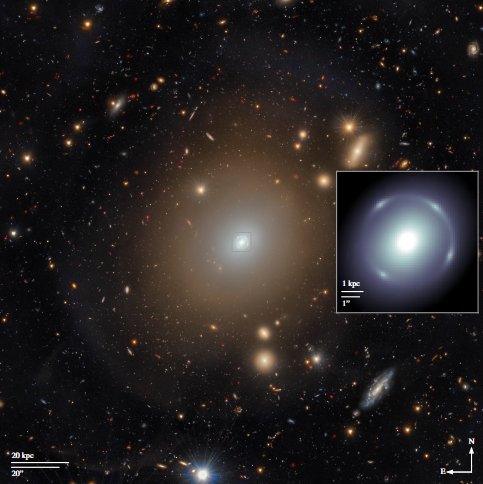
\includegraphics[width=\linewidth]{Immagini/einstein_ring.png}
            \caption{Immagine riprodotta da \textcite{O_Riordan_2025}.}
            \label{fig:einstein_ring}
        \end{figure}
    \end{columns}
\end{frame}

\begin{frame}{I concetti base dello strong gravitational lensing}
    \begin{columns}
        \column{0.3\textwidth}
        \begin{figure}
            \centering
            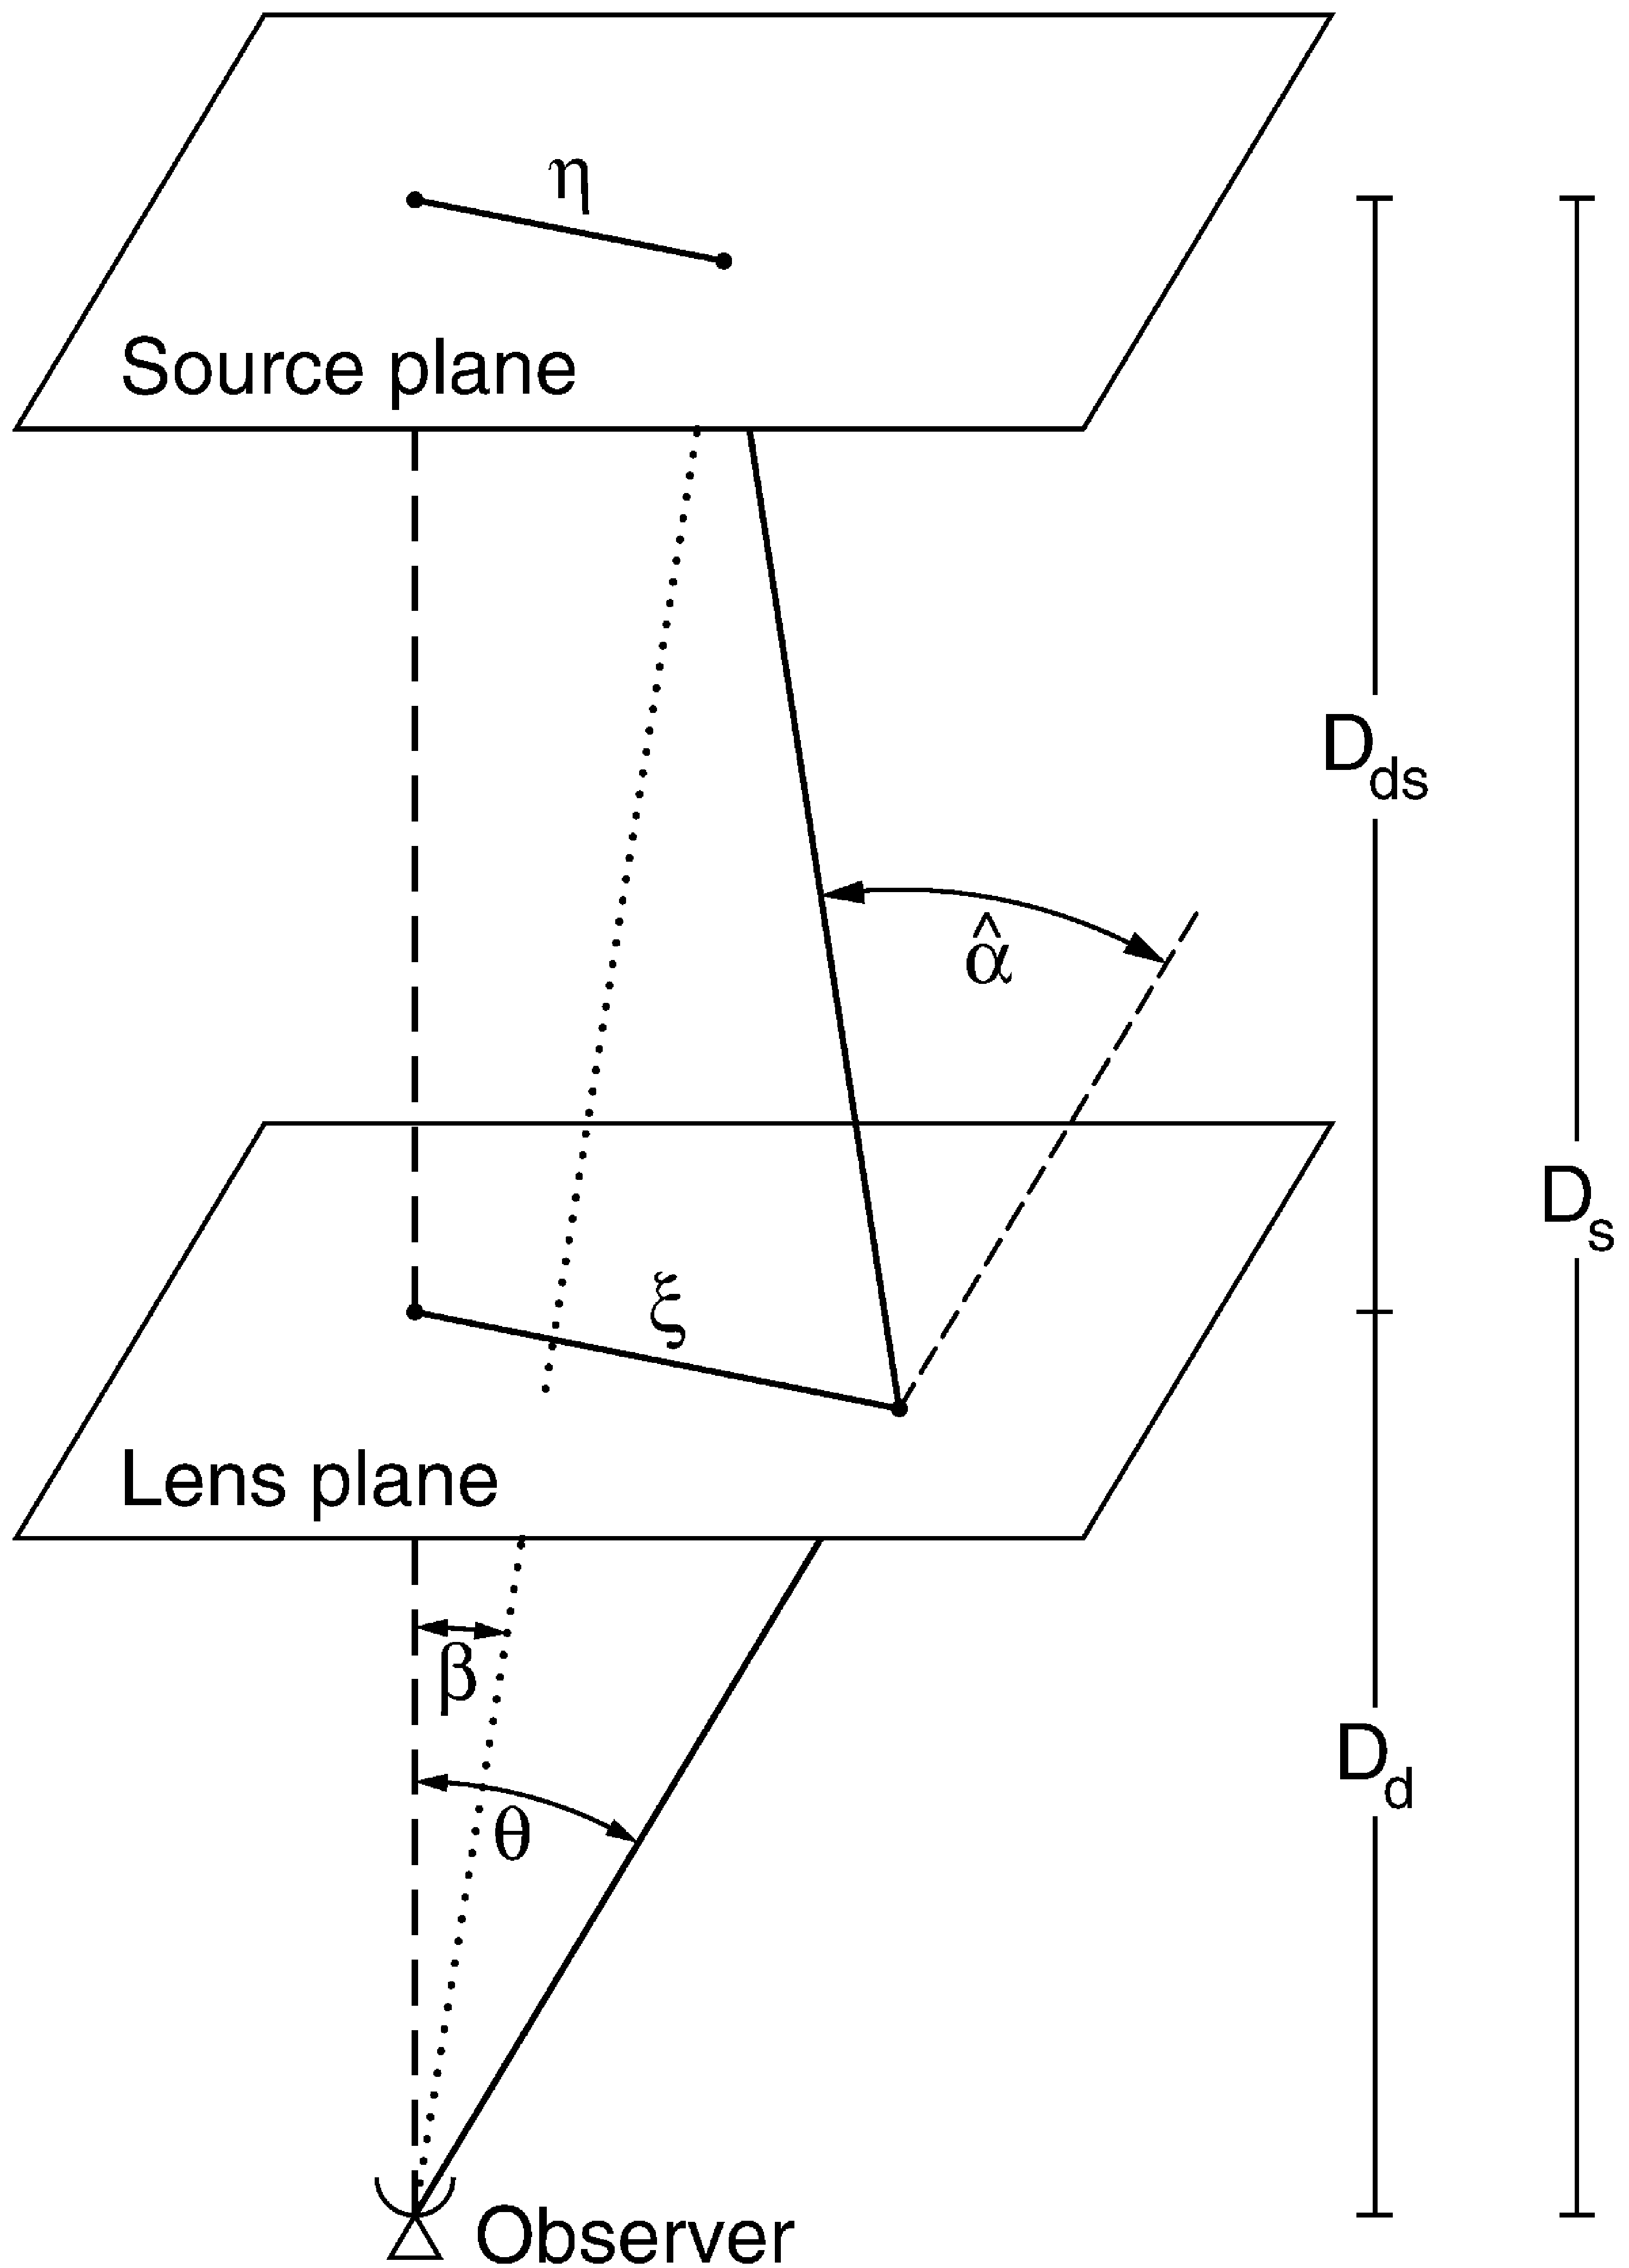
\includegraphics[width=0.75\linewidth]{Immagini/lens-source-planes.png}
            \caption{Immagine riprodotta da \textcite{Bartelmann2001}.}
            \label{fig:source-lens-plane}
        \end{figure}
        \column{0.7\textwidth}
        Grazie all'\emph{approssimazione di lente sottile}, tutta la massa della lente viene proiettata su un piano, detto \textbf{piano della lente}; in maniera analoga, tutta la massa della sorgente viene proiettata sul \textbf{piano della sorgente}.

        Le posizioni angolari sui due piani sono connesse fra loro dall'\emph{equazione della lente}
        \begin{equation*}
            \vec \beta (\vec \theta) = \vec \theta - \hat \alpha (\vec\theta)
        \end{equation*}

        La \emph{convergenza}, indicata puntualmente con $\kappa(\vec\theta)$, misura il potere focalizzante della massa che agisce come lente.

    \end{columns}
\end{frame}

\begin{frame}{Il potenziale della lente e il modello analitico}
    \begin{block}{Definizione}
        Il \textbf{potenziale efficace} della lente è ottenuto proiettando il potenziale gravitazionale tridimensionale lungo la linea di vista, pesando opportunamente rispetto ai parametri geometrici del sistema.
    \end{block}
    Esso contiene tutta l'informazione tutta l'informazione necessaria a descrivere la deflessione gravitazionale ossevata, tra cui la convergenza.

    Il modello di potenziale analitico che descrive meglio le galassie ellittiche e gli ammassi, ovvero le principali lenti forti, è il \textbf{modello isotermo ellittico} (SIE), descritto dal profilo di densità
    \begin{equation*}
        \rho_{SIE}(R)=\frac{\sigma_v^2}{2\pi GR^2}\propto\frac{\theta_E}{R^2}\quad \text{con}\quad  R=\sqrt{\frac{\theta_1^2}{(1-e)}+\theta_2^2(1-e)}
        \label{eq:rho_SIE}
    \end{equation*}
\end{frame}
\begin{frame}{Il lensing come strumento d'indagine della materia oscura}
    Dalle osservabili del lensing gravitazionale forte, la presenza di un sotto-alone si rileva principalmente tramite
    \begin{itemize}
        \item anomalie nei rapporti di flusso;
        \item perturbazioni alla brillanza superficiale.
    \end{itemize}
    Generalmente si formula un \textbf{problema di inferenza bayesiana gerarchica}:
    \begin{enumerate}[1)]
        \item si definisce un modello parametrico;
        \item si stima la distribuzione a posteriori dei parametri;
        \item si trovano i parametri più probabili e si simulano le relative osservazioni;
        \item si confrontano tali immagini con quelle del sistema reale.
    \end{enumerate}
    Poiché la firma delle sotto-strutture non è netta, si usano simulazioni di sistemi controllati per costruire un'intuizione fisica del fenomeno.
\end{frame}

\begin{frame}[plain]
    \begin{figure}
        \centering
        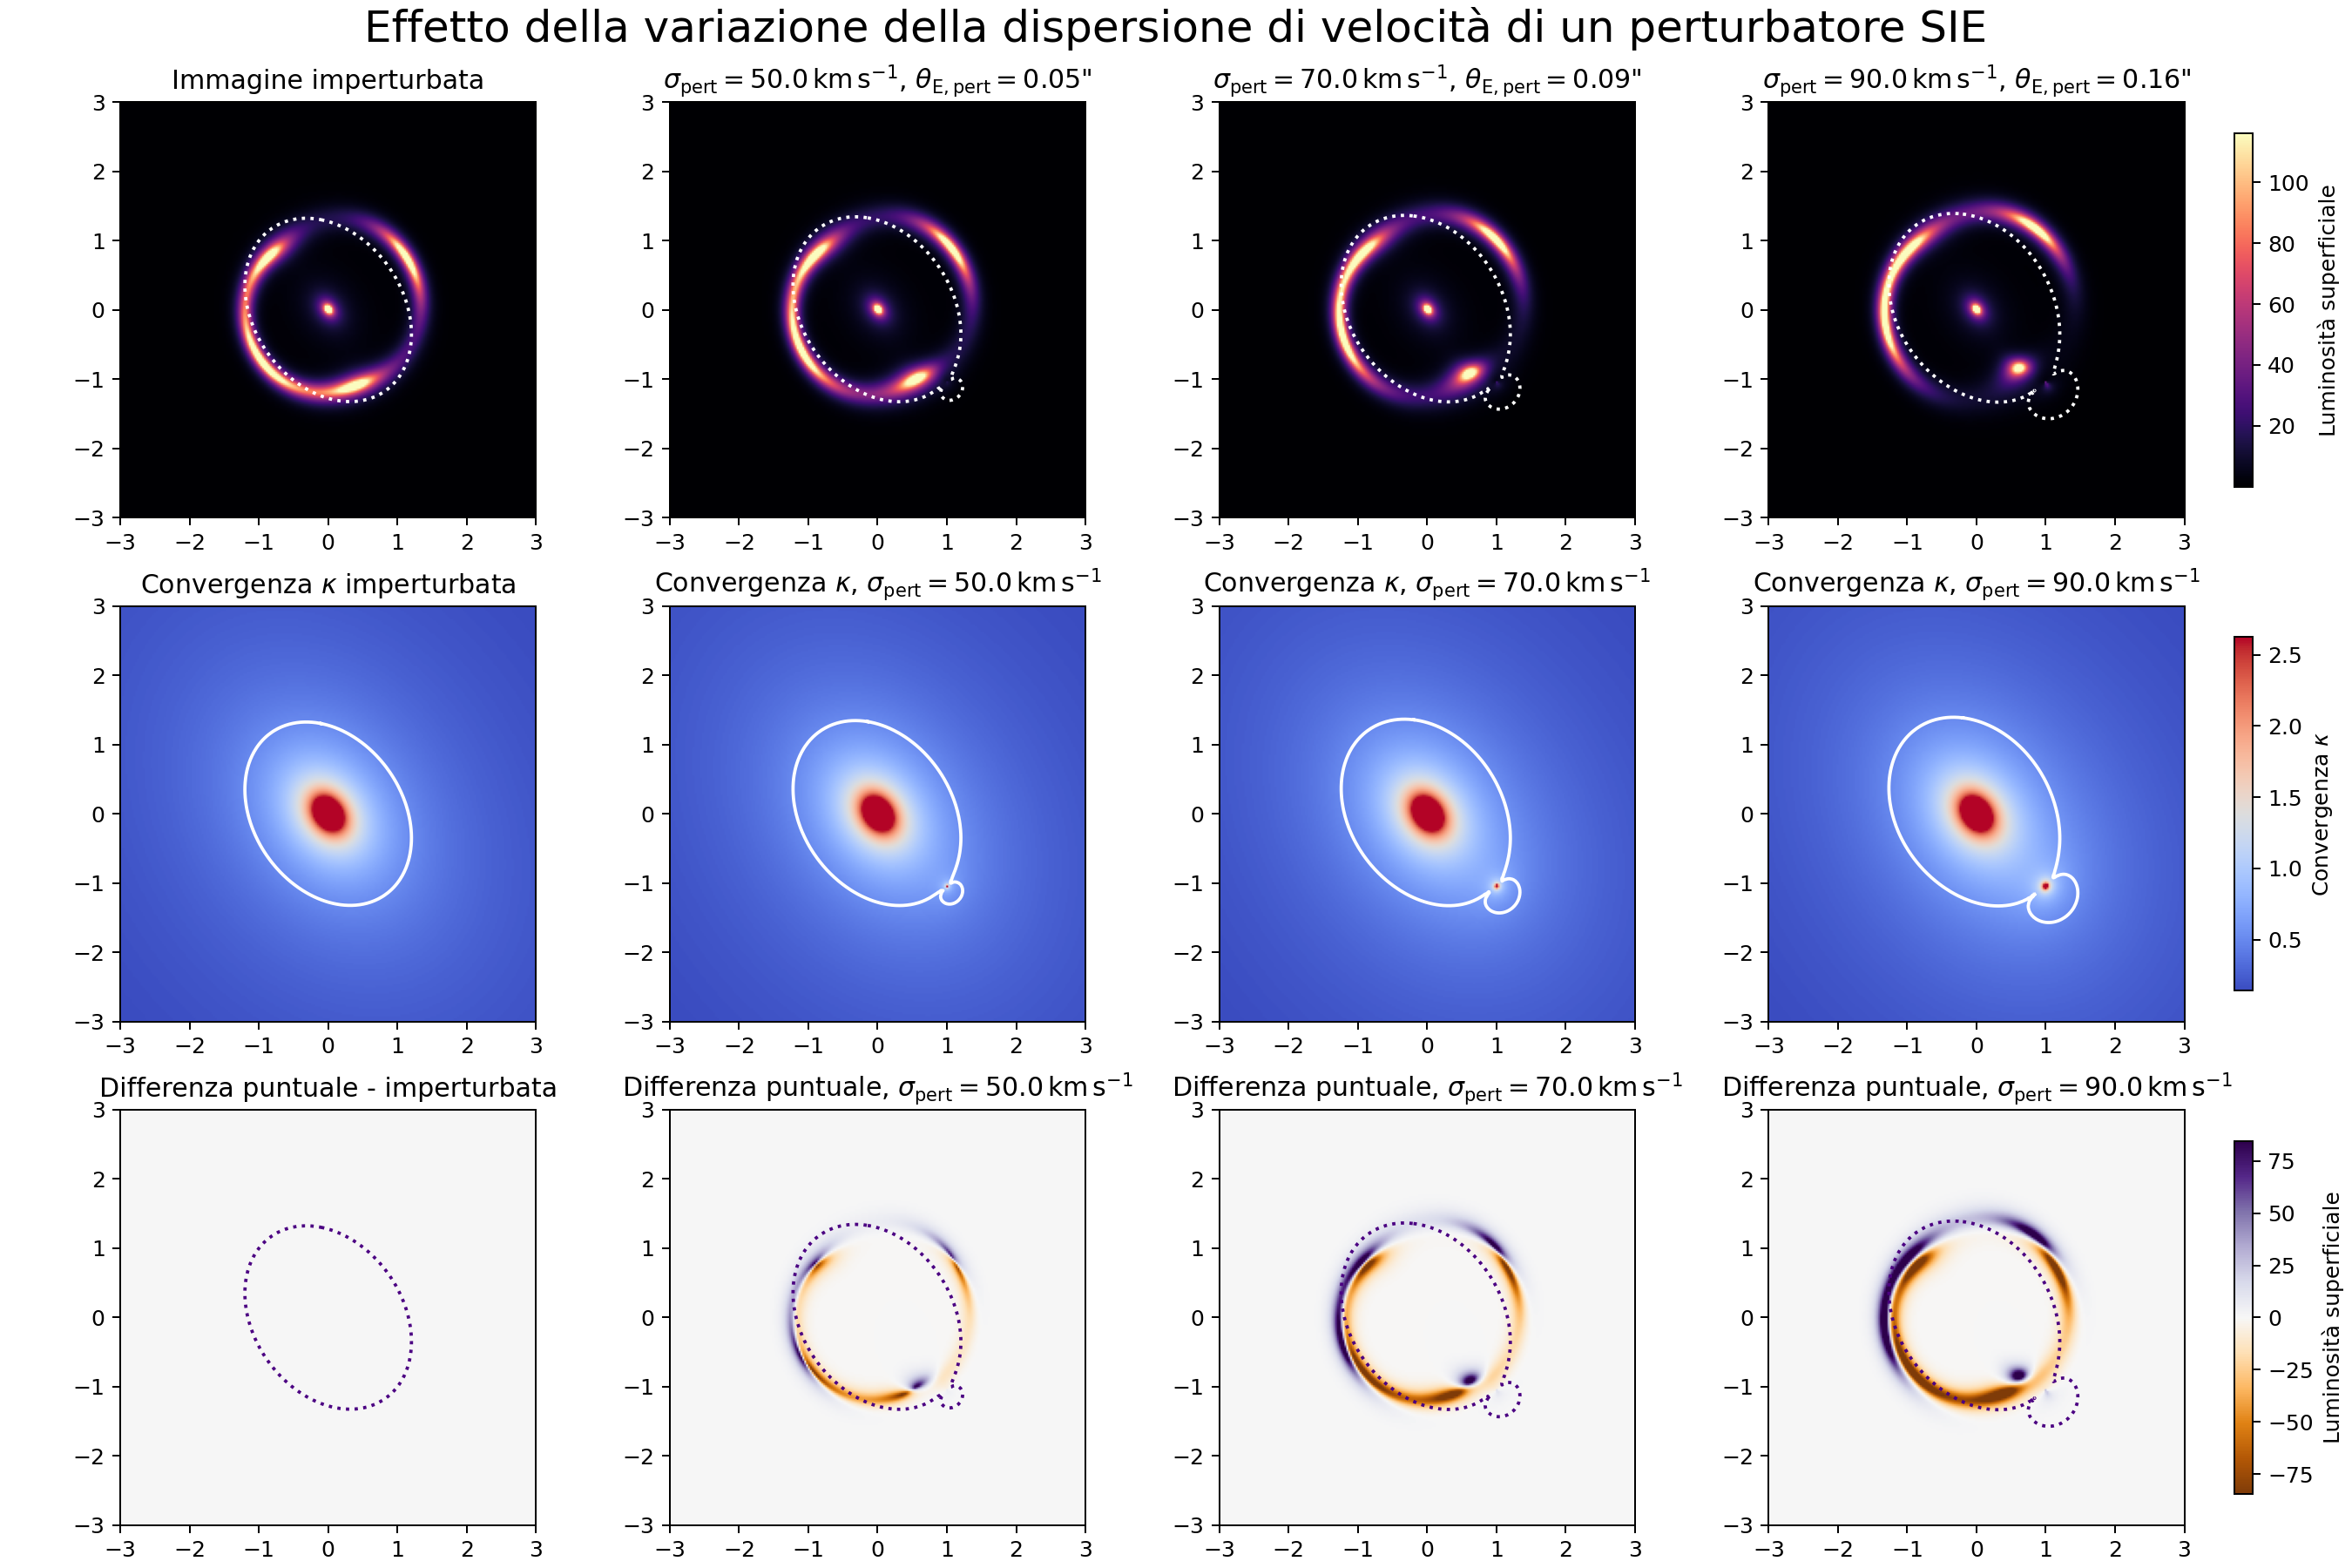
\includegraphics[width=0.9\linewidth]{Immagini/final_simulations_SIE.png}
    \end{figure}
\end{frame}

\begin{frame}[plain]
    \begin{figure}
        \centering
        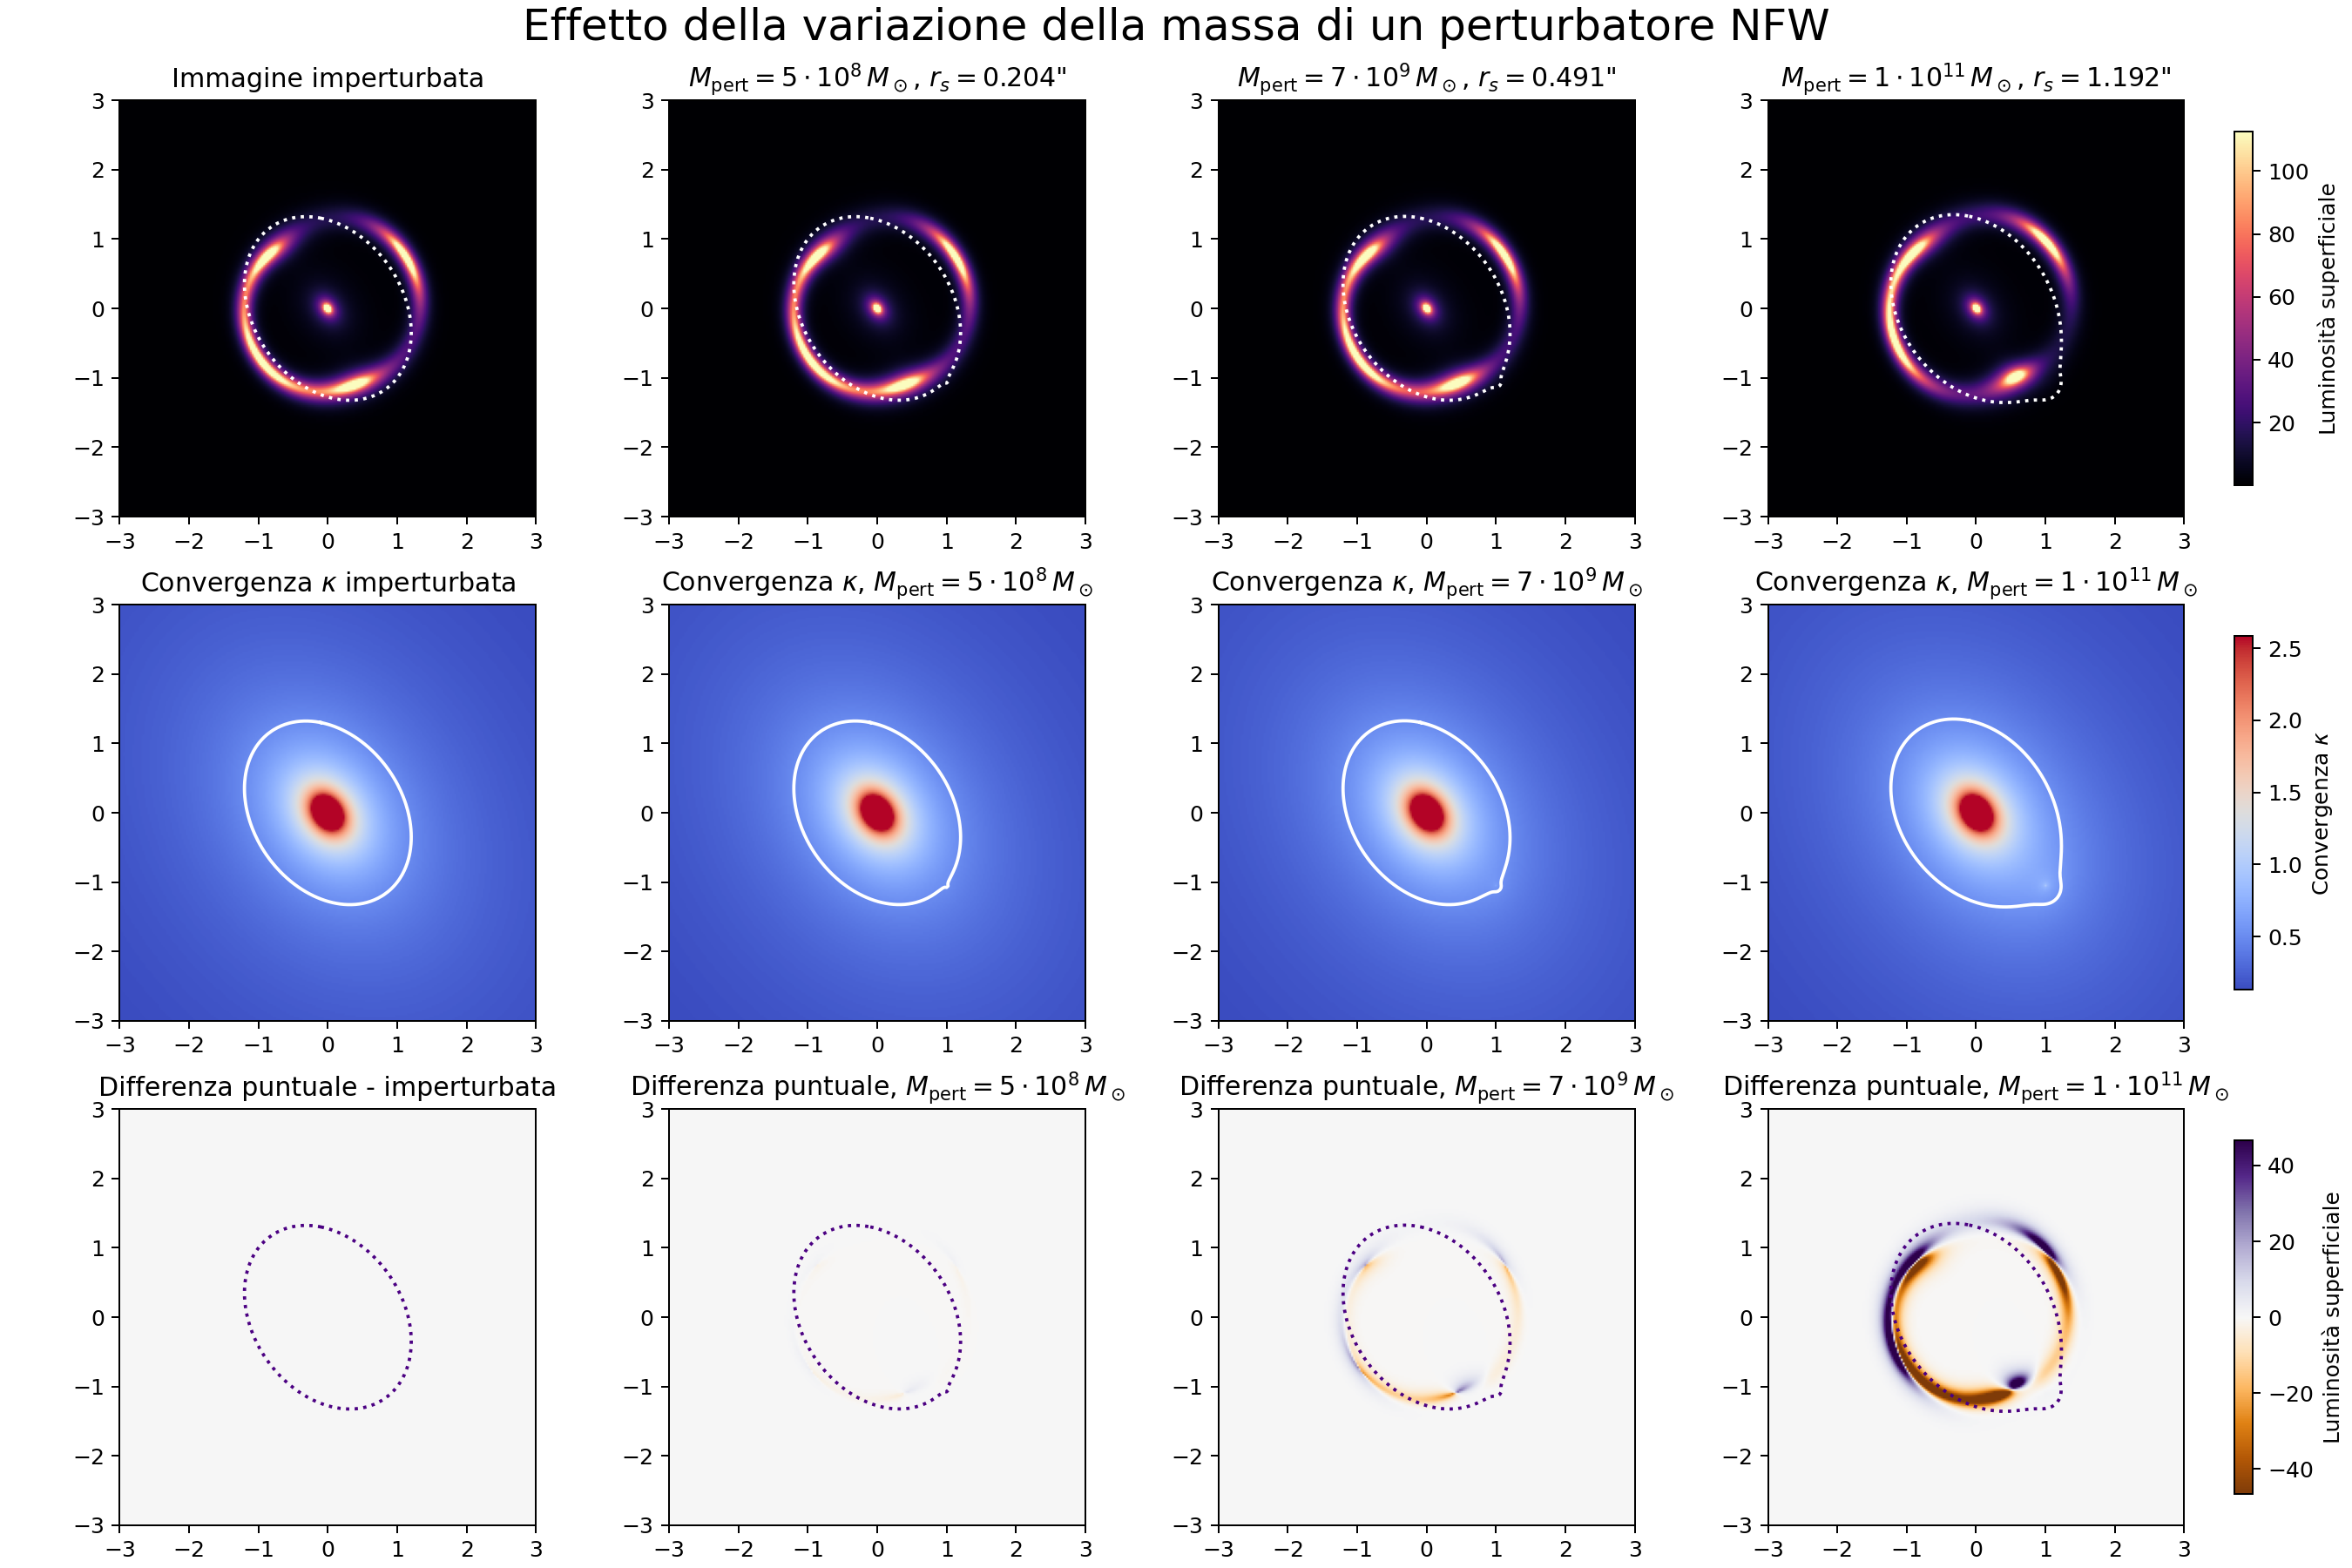
\includegraphics[width=0.9\linewidth]{Immagini/final_simulations_NFW.png}
    \end{figure}
\end{frame}

\begin{frame}{Conclusioni e sviluppi futuri}
    Lo strong gravitational lensing permette di porre vincoli alle proprietà della materia oscura, ma ciò è limitato da
    \begin{itemize}
        \item rumore;
        \item risoluzione strumentale;
        \item complessità dei modelli;
        \item scarsità di sistemi con perturbatori noti.
    \end{itemize}
    Nuove campagne osservative con risoluzioni migliori comprendono \emph{Euclid} e il \emph{Vera Rubin Observatory}.
    La sinergia tra migliori osservazioni e simulazioni più complete permetterà nei prossimi 10 anni di porre vincoli robusti e statisticamente significativi sulla natura della dark matter \parencite{Shajib2024}.

\end{frame}
\begin{frame}{Bibliografia}
    \printbibliography
\end{frame}
\begin{frame}[plain]
    \begin{center}
        \vspace{1.5cm}
        {\color{cobalt!60}\rule{0.3\linewidth}{0.5mm}}
        \vskip0.4cm
        {\usebeamerfont{title}\usebeamercolor[fg]{title}Grazie per l'attenzione!}
        \vskip0.2cm
        {\color{cobalt!60}\rule{0.3\linewidth}{0.5mm}}
    \end{center}
\end{frame}
\end{document}